\documentclass{article}
\usepackage{lmodern}
\usepackage[T1]{fontenc}
\usepackage{shapepar}
\usepackage{microtype}
\usepackage{lipsum}
\usepackage{pgfplots}
\pgfplotsset{compat=1.9}
\usepackage{tikz}
\usetikzlibrary{calc,fit,intersections,folding}
\usepackage{pstricks-add}
\usetikzlibrary{arrows.meta,angles,arrows,quotes,backgrounds,calc}

\usepackage[left = 5mm, right = 5mm]{geometry}

\newcommand{\clrone}{blue}
\newcommand{\clrtwo}{green!70!black}
\newcommand{\clrthree}{red!70!black}

\begin{document}
\thispagestyle{empty}

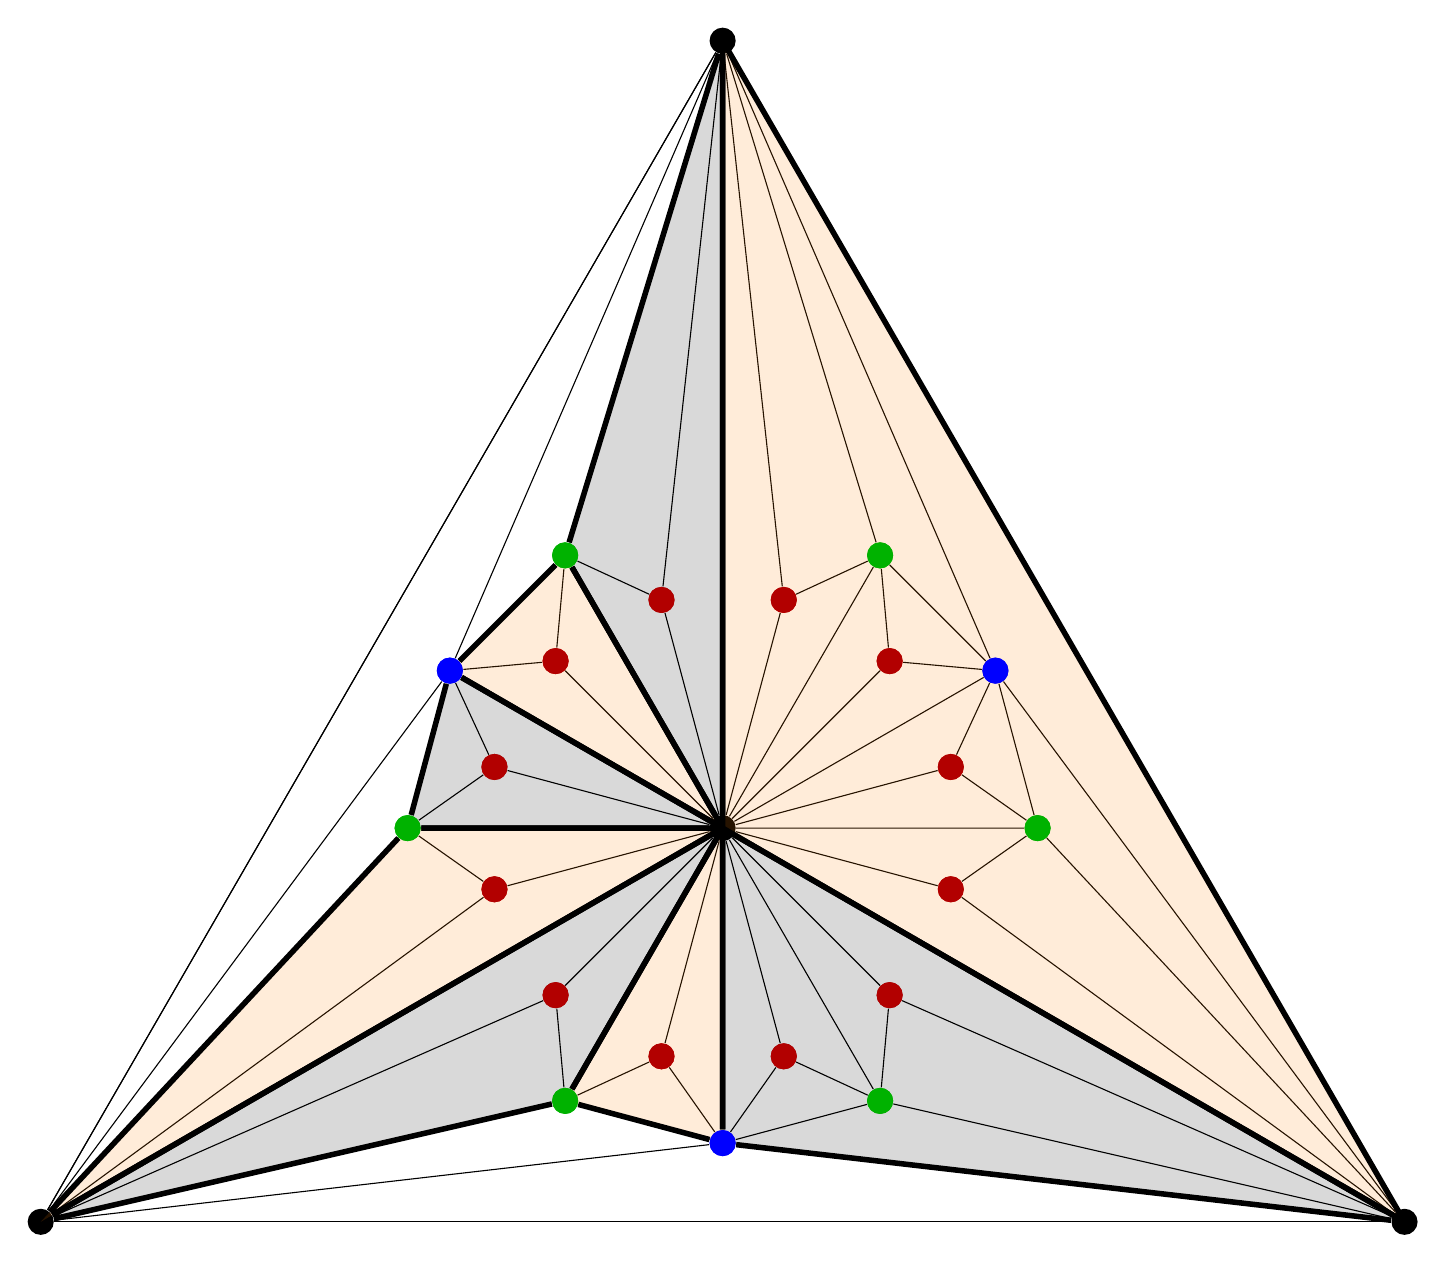
\begin{tikzpicture}[scale = 2]
    \foreach \angle in {0,...,2} {
        \node[fill, circle] (shell\angle) at (90+\angle*120:5) {};
    }
    \node[fill,circle] (shell3) at (0,0) {};
    \foreach \i in {0,...,3} {
        \foreach \j in {0,...,3} {
            \draw[] (shell\i) -- (shell\j);
        }
    }
%gen1
    \foreach \angle in {0,...,2} {
        \node[fill, circle, \clrone] (gen1\angle) at (30+\angle*120:2) {};
    }
    \foreach \i in {0,2,3} {
        \draw[] (shell\i) -- (gen10);
    }
    \foreach \i in {0,1,3} {
        \draw[] (shell\i) -- (gen11);
    }
    \foreach \i in {1,2,3} {
        \draw[] (shell\i) -- (gen12);
    }
%gen2
    \foreach \angle in {0,...,5} {
        \node[fill, circle, \clrtwo] (gen2\angle) at (60+\angle*60:2) {};
    }
    \draw[] (gen20) -- (shell0) (gen20) -- (shell3) (gen20) -- (gen10);
    \draw[] (gen21) -- (shell0) (gen21) -- (shell3) (gen21) -- (gen11);
    \draw[] (gen22) -- (shell1) (gen22) -- (shell3) (gen22) -- (gen11);
    \draw[] (gen23) -- (shell1) (gen23) -- (shell3) (gen23) -- (gen12);
    \draw[] (gen24) -- (shell2) (gen24) -- (shell3) (gen24) -- (gen12);
    \draw[] (gen25) -- (shell2) (gen25) -- (shell3) (gen25) -- (gen10);

    %gen3
    \foreach \angle in {0,...,11} {
        \node[fill, circle, \clrthree] (gen3\angle) at (75+\angle*30:1.5) {};
    }
    \draw[] (gen30) -- (shell3) (gen30) -- (shell0) (gen30) -- (gen20);
    \draw[] (gen31) -- (shell3) (gen31) -- (shell0) (gen31) -- (gen21);
    \draw[] (gen32) -- (shell3) (gen32) -- (gen11) (gen32) -- (gen21);
    \draw[] (gen33) -- (shell3) (gen33) -- (gen11) (gen33) -- (gen22);
    \draw[] (gen34) -- (shell3) (gen34) -- (shell1) (gen34) -- (gen22);
    \draw[] (gen35) -- (shell3) (gen35) -- (shell1) (gen35) -- (gen23);
    \draw[] (gen36) -- (shell3) (gen36) -- (gen12) (gen36) -- (gen23);
    \draw[] (gen37) -- (shell3) (gen37) -- (gen12) (gen37) -- (gen24);
    \draw[] (gen38) -- (shell3) (gen38) -- (shell2) (gen38) -- (gen24);
    \draw[] (gen39) -- (shell3) (gen39) -- (shell2) (gen39) -- (gen25);
    \draw[] (gen310) -- (shell3) (gen310) -- (gen10) (gen310) -- (gen25);
    \draw[] (gen311) -- (shell3) (gen311) -- (gen10) (gen311) -- (gen20);

    \fill[opacity = 0.15, orange] (shell3.center) -- (shell0.center) -- (shell2.center) -- (shell3.center);
    \fill[opacity = 0.15] (shell3.center) -- (gen12.center) -- (shell2.center) -- (shell3.center);
    \fill[opacity = 0.15, orange] (shell3.center) -- (gen23.center) -- (gen12.center) -- (shell3.center);
    \fill[opacity = 0.15] (shell3.center) -- (shell1.center) -- (gen23.center) -- (shell3.center);
    \fill[opacity = 0.15, orange] (shell3.center) -- (gen22.center) -- (shell1.center) -- (shell3.center);
    \fill[opacity = 0.15] (shell3.center) -- (gen11.center) -- (gen22.center) -- (shell3.center);
    \fill[opacity = 0.15, orange] (shell3.center) -- (gen21.center) -- (gen11.center) -- (shell3.center);
    \fill[opacity = 0.15] (shell0.center) -- (gen21.center) -- (shell3.center) -- (shell0.center);
    
    \draw[line width=2pt] (shell3.center) -- (shell0.center) -- (shell2.center) -- (shell3.center);
    \draw[line width=2pt] (shell3.center) -- (gen12) -- (shell2) -- (shell3);
    \draw[line width=2pt] (shell3.center) -- (gen23) -- (gen12) -- (shell3);
    \draw[line width=2pt] (shell3.center) -- (shell1) -- (gen23) -- (shell3);
    \draw[line width=2pt] (shell3.center) -- (gen22) -- (shell1) -- (shell3);
    \draw[line width=2pt] (shell3.center) -- (gen11) -- (gen22) -- (shell3);
    \draw[line width=2pt] (shell3.center) -- (gen21) -- (gen11) -- (shell3);
    \draw[line width=2pt] (shell0) -- (gen21) -- (shell3) -- (shell0);

    \foreach \angle in {0,...,2} {
        \node[fill, circle, \clrone] at (30+\angle*120:2) {};
    }
    \foreach \angle in {0,...,5} {
        \node[fill, circle, \clrtwo] at (60+\angle*60:2) {};
    }
    %gen3
    \foreach \angle in {0,...,11} {
        \node[fill, circle, \clrthree] at (75+\angle*30:1.5) {};
    }
    
\end{tikzpicture}   

\end{document}